\begin{figure}[hbt!]\centering
    \subfloat[]{\label{}
    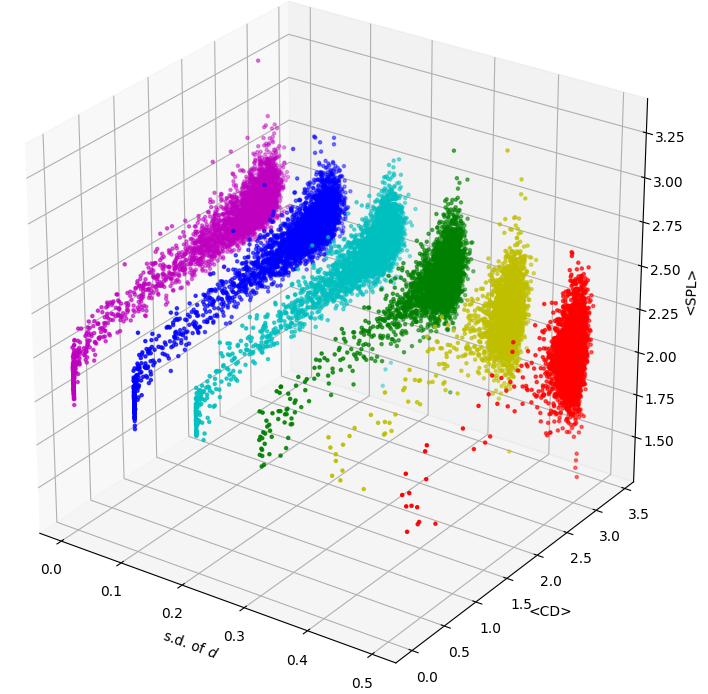
\includegraphics[width=.45\linewidth]{images/base-d.png}}\par

    \subfloat[]{\label{}
    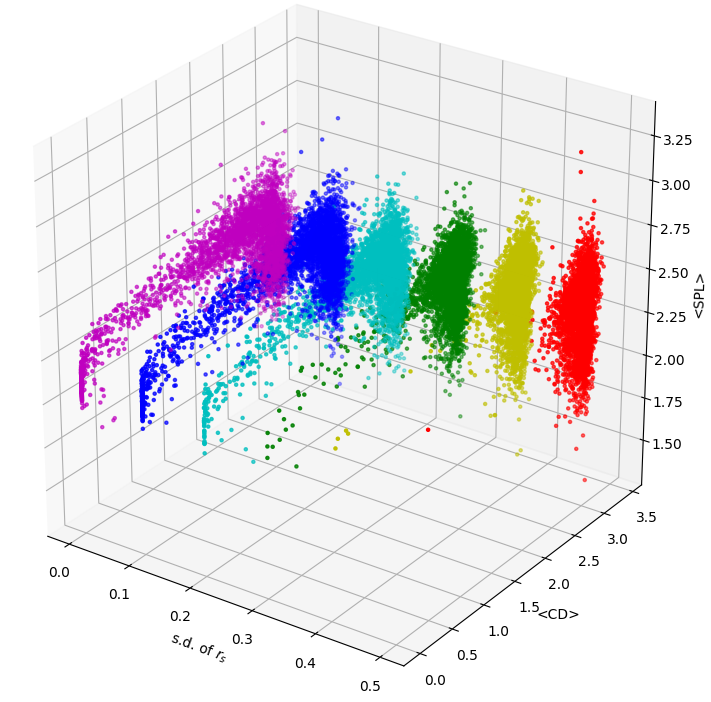
\includegraphics[width=.35\linewidth]{images/base-rs.png}}\hfill
    \subfloat[]{\label{}
    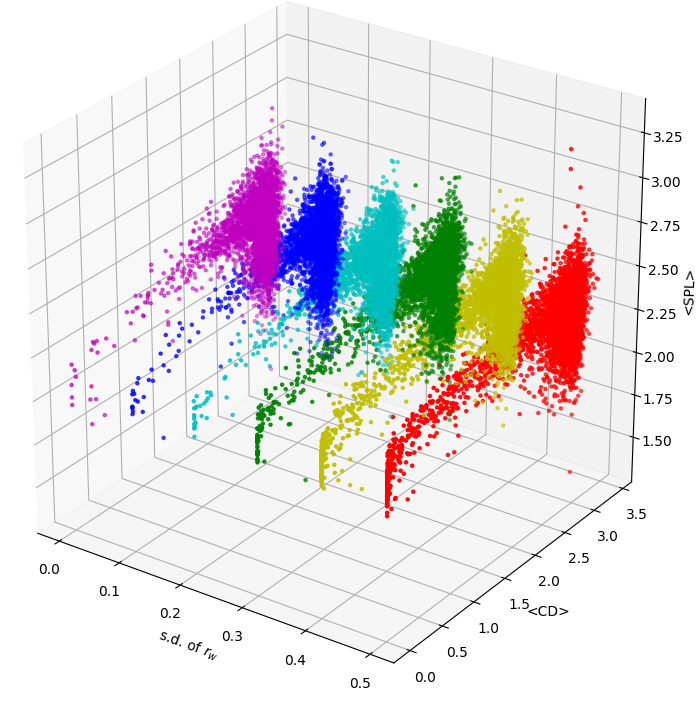
\includegraphics[width=.35\linewidth]{images/base-rw.png}}

    \caption{3D scatter plots showing the effect on SPL and CD of each
    standard deviation of
    (a) $d$, (b) $r_s$ and (c)$r_w$. Each dot is the result of one simulation run, colored
    according to the standard deviation value.}
    \label{figure}
\end{figure}

\section{Replication of Results}\label{sec:confirm}

Figure 1 shows plots for $(<CD>, <SPL)$ plots for standard deviations of
$d$, $r_s$ and $r_w$.
We observe that our desired network configuration, high diversity and
low SPL is achieved for certain parameter settings.
Note that high diversities of cultural tolerance ($d$) and rate of
culture change ($r_s$) help maintain high cultural cultural distance.
In terms of SPL, a high diversity of $d$ helps lower SPL.
These results confirm the results we replicated.



\subsection{Linear Regression}
\begin{gather}\label{eq:base}
    <CD> ~ \thicksim ~ 2.27 + 1.73\sd + 1.85\sr - 2.14\sw -
                5.31\ds + 2.84\dw + 2.86\ssw \label{one}\\
    <SPL> ~ \thicksim ~ 2.47 - 0.66\sd + 0.21\sr - 0.13 \sw -
                0.44\ds + 0.48\dw + 0.18\ssw \label{two}
\end{gather}

The linear terms in equation \eqref{one} show that CD is kept high
when the diversities of $d$ and $r_s$ are high.
CD however is lowered
by a high diversity of $s_w$.
This equation corresponds in form an interpretation to the original paper's
results however, for us the magnitude of each term is lower.
This implies that our experiments yielded less change from an equivalent change
in standard deviations.

In equation \eqref{two}, the most significant factor that decreases SPL is
the standard deviation of cultural tolerance.
In contrast to the equation for CD, our equation corresponds closely to the
same equation in the original paper.

The ANOVA tables in our results also showed that all terms were
extremely statistically significant, confirming the results.